\documentclass{standalone}
\usepackage{tikz}
\usetikzlibrary{patterns, positioning}


\begin{document}
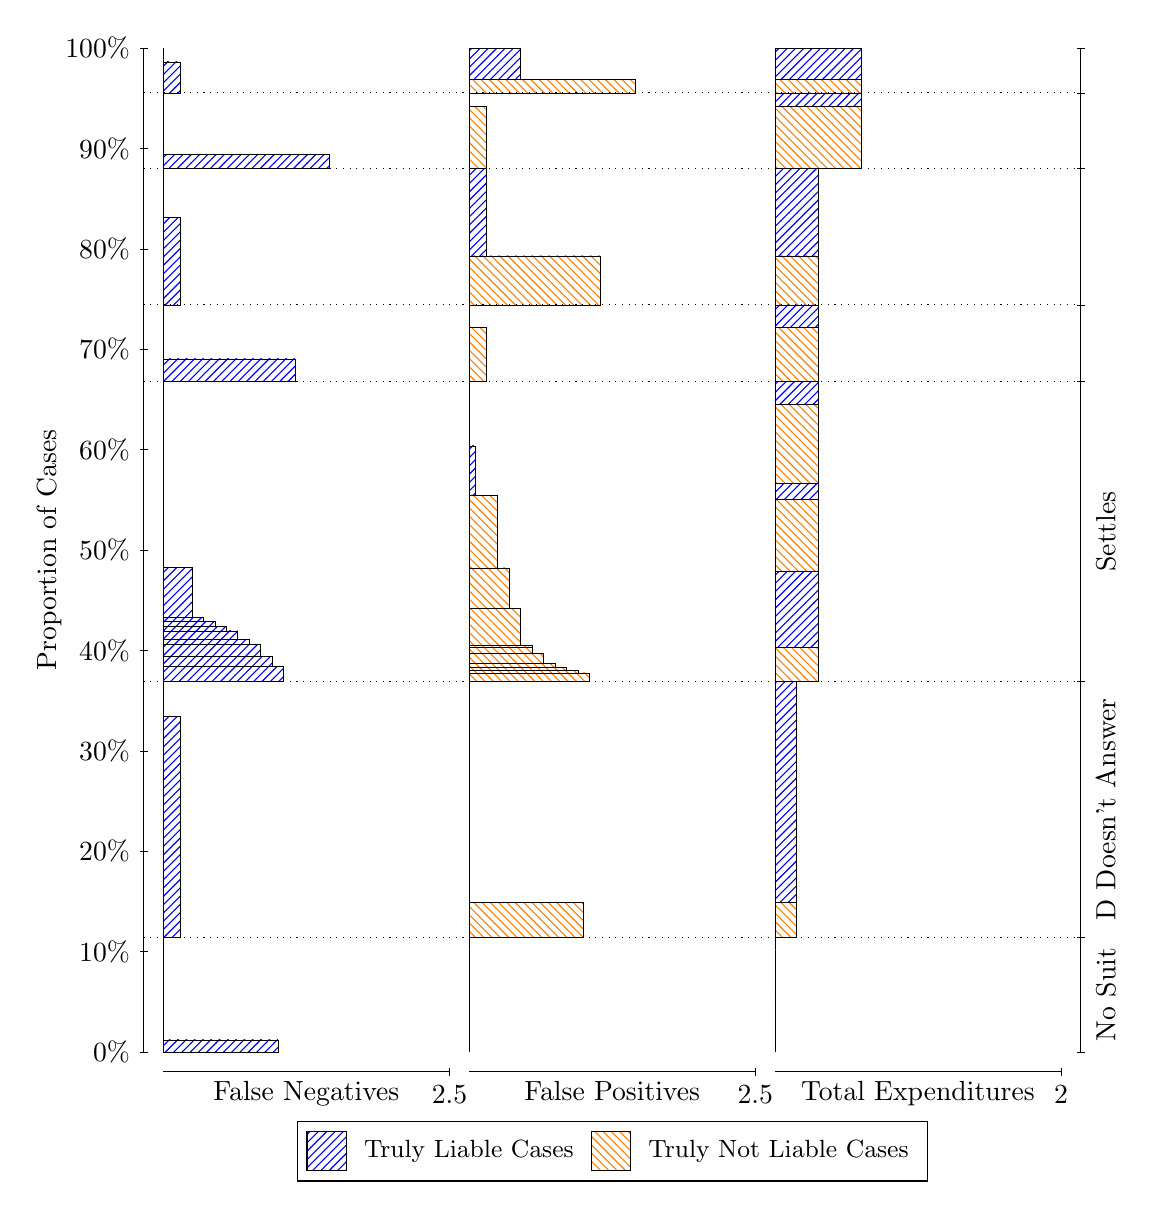
\begin{tikzpicture}
\draw[black, very thin] (1.5,1.75) -- (1.5,14.5);
\node[rotate=90, text=black, anchor=center] at (0.3, 8.125) {Proportion of Cases};
\draw[black, very thin] (1.45,1.75) -- (1.55,1.75);
\node[text=black, anchor=east] at (1.45, 1.75) {0\%};
\draw[black, very thin] (1.45,3.025) -- (1.55,3.025);
\node[text=black, anchor=east] at (1.45, 3.025) {10\%};
\draw[black, very thin] (1.45,4.3) -- (1.55,4.3);
\node[text=black, anchor=east] at (1.45, 4.3) {20\%};
\draw[black, very thin] (1.45,5.575) -- (1.55,5.575);
\node[text=black, anchor=east] at (1.45, 5.575) {30\%};
\draw[black, very thin] (1.45,6.85) -- (1.55,6.85);
\node[text=black, anchor=east] at (1.45, 6.85) {40\%};
\draw[black, very thin] (1.45,8.125) -- (1.55,8.125);
\node[text=black, anchor=east] at (1.45, 8.125) {50\%};
\draw[black, very thin] (1.45,9.4) -- (1.55,9.4);
\node[text=black, anchor=east] at (1.45, 9.4) {60\%};
\draw[black, very thin] (1.45,10.675) -- (1.55,10.675);
\node[text=black, anchor=east] at (1.45, 10.675) {70\%};
\draw[black, very thin] (1.45,11.95) -- (1.55,11.95);
\node[text=black, anchor=east] at (1.45, 11.95) {80\%};
\draw[black, very thin] (1.45,13.225) -- (1.55,13.225);
\node[text=black, anchor=east] at (1.45, 13.225) {90\%};
\draw[black, very thin] (1.45,14.5) -- (1.55,14.5);
\node[text=black, anchor=east] at (1.45, 14.5) {100\%};

\draw[black, very thin] (13.4,1.75) -- (13.4,14.5);
\draw[black, very thin] (13.35,1.75) -- (13.45,1.75);
\node[anchor=west] at (13.35, 1.75) {};
\draw[black, very thin] (13.35,3.2067) -- (13.45,3.2067);
\node[anchor=west] at (13.35, 3.2067) {};
\draw[black, very thin] (13.35,6.452) -- (13.45,6.452);
\node[anchor=west] at (13.35, 6.452) {};
\draw[black, very thin] (13.35,10.268) -- (13.45,10.268);
\node[anchor=west] at (13.35, 10.268) {};
\draw[black, very thin] (13.35,11.239) -- (13.45,11.239);
\node[anchor=west] at (13.35, 11.239) {};
\draw[black, very thin] (13.35,12.97) -- (13.45,12.97);
\node[anchor=west] at (13.35, 12.97) {};
\draw[black, very thin] (13.35,13.931) -- (13.45,13.931);
\node[anchor=west] at (13.35, 13.931) {};
\draw[black, very thin] (13.35,14.5) -- (13.45,14.5);
\node[anchor=west] at (13.35, 14.5) {};

\draw[black, very thin, pattern color=blue, pattern=north east lines] (1.75,1.75) rectangle (3.2033,1.9033);
\draw[black, very thin, pattern color=orange, pattern=north west lines] (1.75,1.9033) rectangle (1.75,3.2067);
\draw[black, very thin, pattern color=blue, pattern=north east lines] (1.75,3.2067) rectangle (1.968,6.0125);
\draw[black, very thin, pattern color=orange, pattern=north west lines] (1.75,6.0125) rectangle (1.75,6.452);
\draw[black, very thin, pattern color=blue, pattern=north east lines] (1.75,6.452) rectangle (3.276,6.6473);
\draw[black, very thin, pattern color=blue, pattern=north east lines] (1.75,6.6473) rectangle (3.1307,6.776);
\draw[black, very thin, pattern color=blue, pattern=north east lines] (1.75,6.776) rectangle (2.9853,6.9295);
\draw[black, very thin, pattern color=blue, pattern=north east lines] (1.75,6.9295) rectangle (2.84,6.9878);
\draw[black, very thin, pattern color=blue, pattern=north east lines] (1.75,6.9878) rectangle (2.6947,7.0965);
\draw[black, very thin, pattern color=blue, pattern=north east lines] (1.75,7.0965) rectangle (2.5493,7.1574);
\draw[black, very thin, pattern color=blue, pattern=north east lines] (1.75,7.1574) rectangle (2.404,7.2202);
\draw[black, very thin, pattern color=blue, pattern=north east lines] (1.75,7.2202) rectangle (2.2587,7.2724);
\draw[black, very thin, pattern color=blue, pattern=north east lines] (1.75,7.2724) rectangle (2.1133,7.9021);
\draw[black, very thin, pattern color=orange, pattern=north west lines] (1.75,7.9021) rectangle (1.75,10.268);
\draw[black, very thin, pattern color=blue, pattern=north east lines] (1.75,10.268) rectangle (3.4213,10.553);
\draw[black, very thin, pattern color=orange, pattern=north west lines] (1.75,10.553) rectangle (1.75,11.239);
\draw[black, very thin, pattern color=blue, pattern=north east lines] (1.75,11.239) rectangle (1.968,12.347);
\draw[black, very thin, pattern color=orange, pattern=north west lines] (1.75,12.347) rectangle (1.75,12.97);
\draw[black, very thin, pattern color=blue, pattern=north east lines] (1.75,12.97) rectangle (3.8573,13.147);
\draw[black, very thin, pattern color=orange, pattern=north west lines] (1.75,13.147) rectangle (1.75,13.931);
\draw[black, very thin, pattern color=blue, pattern=north east lines] (1.75,13.931) rectangle (1.968,14.325);
\draw[black, very thin, pattern color=orange, pattern=north west lines] (1.75,14.325) rectangle (1.75,14.5);
\draw[black, very thin, pattern color=orange, pattern=north west lines] (5.6333,1.75) rectangle (5.6333,3.0535);
\draw[black, very thin, pattern color=blue, pattern=north east lines] (5.6333,3.0535) rectangle (5.6333,3.2067);
\draw[black, very thin, pattern color=orange, pattern=north west lines] (5.6333,3.2067) rectangle (7.0867,3.6462);
\draw[black, very thin, pattern color=blue, pattern=north east lines] (5.6333,3.6462) rectangle (5.6333,6.452);
\draw[black, very thin, pattern color=orange, pattern=north west lines] (5.6333,6.452) rectangle (7.1593,6.5653);
\draw[black, very thin, pattern color=orange, pattern=north west lines] (5.6333,6.5653) rectangle (7.014,6.5944);
\draw[black, very thin, pattern color=orange, pattern=north west lines] (5.6333,6.5944) rectangle (6.8687,6.6327);
\draw[black, very thin, pattern color=orange, pattern=north west lines] (5.6333,6.6327) rectangle (6.7233,6.6877);
\draw[black, very thin, pattern color=orange, pattern=north west lines] (5.6333,6.6877) rectangle (6.578,6.8128);
\draw[black, very thin, pattern color=orange, pattern=north west lines] (5.6333,6.8128) rectangle (6.4327,6.8928);
\draw[black, very thin, pattern color=orange, pattern=north west lines] (5.6333,6.8928) rectangle (6.4327,6.9183);
\draw[black, very thin, pattern color=orange, pattern=north west lines] (5.6333,6.9183) rectangle (6.2873,7.3858);
\draw[black, very thin, pattern color=orange, pattern=north west lines] (5.6333,7.3858) rectangle (6.142,7.8977);
\draw[black, very thin, pattern color=orange, pattern=north west lines] (5.6333,7.8977) rectangle (5.9967,8.8175);
\draw[black, very thin, pattern color=blue, pattern=north east lines] (5.6333,8.8175) rectangle (5.706,9.4471);
\draw[black, very thin, pattern color=blue, pattern=north east lines] (5.6333,9.4471) rectangle (5.6333,10.268);
\draw[black, very thin, pattern color=orange, pattern=north west lines] (5.6333,10.268) rectangle (5.8513,10.953);
\draw[black, very thin, pattern color=blue, pattern=north east lines] (5.6333,10.953) rectangle (5.6333,11.239);
\draw[black, very thin, pattern color=orange, pattern=north west lines] (5.6333,11.239) rectangle (7.3047,11.861);
\draw[black, very thin, pattern color=blue, pattern=north east lines] (5.6333,11.861) rectangle (5.8513,12.97);
\draw[black, very thin, pattern color=orange, pattern=north west lines] (5.6333,12.97) rectangle (5.8513,13.754);
\draw[black, very thin, pattern color=blue, pattern=north east lines] (5.6333,13.754) rectangle (5.6333,13.931);
\draw[black, very thin, pattern color=orange, pattern=north west lines] (5.6333,13.931) rectangle (7.7407,14.105);
\draw[black, very thin, pattern color=blue, pattern=north east lines] (5.6333,14.105) rectangle (6.2873,14.5);
\draw[black, very thin, pattern color=orange, pattern=north west lines] (9.5167,1.75) rectangle (9.5167,3.0535);
\draw[black, very thin, pattern color=blue, pattern=north east lines] (9.5167,3.0535) rectangle (9.5167,3.2067);
\draw[black, very thin, pattern color=orange, pattern=north west lines] (9.5167,3.2067) rectangle (9.7892,3.6462);
\draw[black, very thin, pattern color=blue, pattern=north east lines] (9.5167,3.6462) rectangle (9.7892,6.452);
\draw[black, very thin, pattern color=orange, pattern=north west lines] (9.5167,6.452) rectangle (10.062,6.8928);
\draw[black, very thin, pattern color=blue, pattern=north east lines] (9.5167,6.8928) rectangle (10.062,7.8526);
\draw[black, very thin, pattern color=orange, pattern=north west lines] (9.5167,7.8526) rectangle (10.062,8.7723);
\draw[black, very thin, pattern color=blue, pattern=north east lines] (9.5167,8.7723) rectangle (10.062,8.9676);
\draw[black, very thin, pattern color=orange, pattern=north west lines] (9.5167,8.9676) rectangle (10.062,9.9725);
\draw[black, very thin, pattern color=blue, pattern=north east lines] (9.5167,9.9725) rectangle (10.062,10.268);
\draw[black, very thin, pattern color=orange, pattern=north west lines] (9.5167,10.268) rectangle (10.062,10.953);
\draw[black, very thin, pattern color=blue, pattern=north east lines] (9.5167,10.953) rectangle (10.062,11.239);
\draw[black, very thin, pattern color=orange, pattern=north west lines] (9.5167,11.239) rectangle (10.062,11.861);
\draw[black, very thin, pattern color=blue, pattern=north east lines] (9.5167,11.861) rectangle (10.062,12.97);
\draw[black, very thin, pattern color=orange, pattern=north west lines] (9.5167,12.97) rectangle (10.607,13.754);
\draw[black, very thin, pattern color=blue, pattern=north east lines] (9.5167,13.754) rectangle (10.607,13.931);
\draw[black, very thin, pattern color=orange, pattern=north west lines] (9.5167,13.931) rectangle (10.607,14.105);
\draw[black, very thin, pattern color=blue, pattern=north east lines] (9.5167,14.105) rectangle (10.607,14.5);
\draw[black, dotted] (1.5,3.2067) -- (13.4,3.2067);
\draw[black, dotted] (1.5,6.452) -- (13.4,6.452);
\draw[black, dotted] (1.5,10.268) -- (13.4,10.268);
\draw[black, dotted] (1.5,11.239) -- (13.4,11.239);
\draw[black, dotted] (1.5,12.97) -- (13.4,12.97);
\draw[black, dotted] (1.5,13.931) -- (13.4,13.931);
\draw[black, very thin] (1.75,1.5) -- (5.3833,1.5);
\node[text=black, anchor=north] at (3.5667, 1.5) {False Negatives};
\draw[black, very thin] (5.3833,1.45) -- (5.3833,1.55);
\node[text=black, anchor=north] at (5.3833, 1.45) {2.5};

\draw[black, very thin] (5.6333,1.5) -- (9.2667,1.5);
\node[text=black, anchor=north] at (7.45, 1.5) {False Positives};
\draw[black, very thin] (9.2667,1.45) -- (9.2667,1.55);
\node[text=black, anchor=north] at (9.2667, 1.45) {2.5};

\draw[black, very thin] (9.5167,1.5) -- (13.15,1.5);
\node[text=black, anchor=north] at (11.333, 1.5) {Total Expenditures};
\draw[black, very thin] (13.15,1.45) -- (13.15,1.55);
\node[text=black, anchor=north] at (13.15, 1.45) {2};

\node[text=black, centered, rotate=90] at (13.72, 2.4784) {No Suit};
\node[text=black, centered, rotate=90] at (13.72, 4.8294) {D Doesn't Answer};
\node[text=black, centered, rotate=90] at (13.72, 8.3598) {Settles};





\draw (7.449999999999999,1.5) node[draw=none] (baseCoordinate) {};
\begin{scope}[align=center]
        \matrix[scale=0.5, draw=black, below=0.5cm of baseCoordinate, nodes={draw}, column sep=0.1cm]{
            \node[rectangle, draw, minimum width=0.5cm, minimum height=0.5cm, pattern color=blue, pattern=north east lines] {}; &
            \node[draw=none, font=\small, text=black] (B) {Truly Liable Cases}; &
            \node[rectangle, draw, minimum width=0.5cm, minimum height=0.5cm, pattern color=orange, pattern=north west lines] {}; &
            \node[draw=none, font=\small, text=black] (B) {Truly Not Liable Cases}; \\
            };
\end{scope}

\end{tikzpicture}
\end{document}